\documentclass[11pt, oneside]{article}   	% use "amsart" instead of "article" for AMSLaTeX format
\usepackage{geometry}                		% See geometry.pdf to learn the layout options. There are lots.
\geometry{letterpaper}                   		% ... or a4paper or a5paper or ... 
%\geometry{landscape}                		% Activate for for rotated page geometry
%\usepackage[parfill]{parskip}    		% Activate to begin paragraphs with an empty line rather than an indent
\usepackage{graphicx}				% Use pdf, png, jpg, or eps§ with pdflatex; use eps in DVI mode
								% TeX will automatically convert eps --> pdf in pdflatex		
\usepackage{amssymb}

\title{Amplicon sequencing (16S and ITS) processing platform}
\author{Thomas Gurry - thomasgurry@gmail.com}
\date{}							% Activate to display a given date or no date

\begin{document}
\maketitle
\section{Introduction}
This document describes the process of going from raw 16S or ITS data to processed data (OTU tables, oligotypes, etc.).  This is orchestrated by the script {\tt raw2otu.py}.  The platform is designed in such a manner that the user interfaces with a single script, {\tt Master.py}, which takes as input the path to the folder containing the dataset.  Each dataset folder must contain a machine-readable text file, called a summary file, which gives instructions to {\tt Master.py}.  The format of these summary files, and all files required for 16S or ITS processing, are described in the section below.

\section{Preparing your dataset for processing}
\subsection{Raw FASTQ files}
FASTQ files have different ASCII encodings for the quality characters.  It is often ASCII base 33 or ASCII base 64.  Check this using {\tt usearch -fastq\_chars yourFASTQfile.fastq} and specify the encoding in the summary file.  If left unspecified, it will default to base 33.

The pipeline is designed to take a single FASTQ file, multiple FASTQ files in which each file corresponds to one sample, a single FASTA file with barcodes and primers removed, and multiple FASTA files in which each file corresponds to one sample. FASTQ files may contain primers and/or barcodes or may have them removed. All configurations and processing requirements are specified through the summary file.

\subsection{Metadata}
Metadata is uploaded as is to S3 for storage with the raw data.  Ideally, we want to capture as much of the metadata as possible in the database and into file objects describing the data (e.g. OTU tables in BIOM format).  We can produce a file with three columns: {\tt sample\_ID}, {\tt disease\_label} and {\tt keywords}.  {\tt sample\_ID} corresponds to the name ID of the sample as is listed in the OTU table.  {\tt disease\_label} is a specific label used for each subject and can be more general than disease.  Note that none of these metadata are currently used by the pipeline, so you can process your data without knowing anything other than the sample barcode.  This format is merely recommended to facilitate standardized storage and of course necessary for downstream analysis.

\subsection{Summary files}
This file, named {\tt summary\_file.txt}, is a machine-readable, \textbf{tab-delimited} file that must accompany any dataset directory when uploaded to the cloud.  It should be found in the highest directory level for the dataset directory in the S3 bucket.  It is a text file with descriptors for the data and paths to all relevant datafiles within the directory.  It can include a True or False flag for whether any associated raw 16S/ITS data has already been processed.  

The order in which items are listed between the lines {\tt \#16S\_start} and {\tt \#16S\_end} (for 16S) and between lines {\tt \#ITS\_start} and {\tt \#ITS\_end} (for ITS) does not matter.  

Note that any white space in the summary file examples below corresponds to a single tab character.

\subsubsection{List of 16S and ITS attributes}
See the table at the end of this document.
\begin{table}[h!]
  \begin{center}
    \label{tab:table1}
    \begin{tabular}{| c | c |}
    \hline
      \textbf{Attribute} & \textbf{Description} \\
      \hline
      {\tt RAW\_FASTQ\_FILE} & Raw FASTQ file name/path within the dataset directory \\
      \hline
      {\tt RAW\_FASTA\_FILE} & Raw FASTA file name/path if raw data is in FASTA format \\
      \hline
      {\tt RAW\_FASTQ\_FILES}
       & For demultiplexed datasets where samples are separated \\
       & into separate FASTQ files.  Filename of two column file \\
       & containing FASTQ filenames in first column and sample IDs \\
       & in the second column. \\
       \hline
      {\tt RAW\_FASTA\_FILES} 
       & For demultiplexed datasets where samples are separated \\
       & into separate FASTA files.  Filename of two column file \\
       & containing FASTA filenames in first column and sample IDs \\
       & in the second column. \\
       \hline
      {\tt ASCII\_ENCODING} & ASCII quality encoding in FASTQ.  Supports either \\
       & 'ASCII\_BASE\_33'  or 'ASCII\_BASE\_64'.  Set to 33 if unspecified. \\
       \hline
      {\tt PRIMERS\_FILE} & Filename/path to primers file. \\
       & {\tt required}: If primers have already been removed, specify 'None'. \\
       \hline
      {\tt BARCODES\_MAP} & Filename/path to barcodes map file. \\
       & {\tt required}: If barcodes have already been removed, specify 'None'. \\
       \hline
      {\tt BARCODES\_MODE} & '1' = barcodes in sequence ID, \\
       &  '2' = barcodes in sequences themselves. \\
       \hline
       {\tt BARCODES\_SEPARATOR} & Separator character.  See description in Case 2 below. \\
       \hline
       {\tt METADATA\_FILE} & Filename/path to metadata file. \\
       \hline
       {\tt PROCESSED} & True/False flag for whether data have already been processed. \\
        & {\tt required}: Set to 'False' for processing to proceed. \\
        \hline
        {\tt TRIM\_LENGTH} & Length to which all sequences should be trimmed.  \\
        & Defaults to 101 if unspecified. \\
        \hline
        {\tt QUALITY\_TRIM} & Minimum quality score allowed.  \\
        & Sequences are truncated at the first base having quality \\
        & score < {\tt value}.  Defaults to 25 if unspecified. \\
        \hline
		{\tt MAX\_ERRORS} & Maximum expected errors allowed. \\
		& After length trimming, sequences with more than {\tt MAX\_ERRORS} \\
		& expected errors are discarded. If not specified or if a {\tt TRIM\_QUALITY} value \\
		& is specified, defaults to quality trimming behavior, above. \\
		\hline
        {\tt MIN\_COUNT} & Minimum sequence count in dereplication across \\
        & all samples.  Defaults to 10 if unspecified (i.e. sequences with fewer than  \\
        & 10 occurrences in the entire dataset will not be considered downstream). \\
        \hline
        {\tt OTU\_SIMILARITY} & Integer specifying the percent similarity desired \\
         &  in OTU clustering.  Defaults to 97 if unspecified. \\
	\hline
	{\tt RDP\_CUTOFF} & Desired probability cut-off for Ribosomal Database Project \\
	& assignments.  Assignments at each taxonomic level will be evaluated and \\
	& those with a lower probability than this cutoff will be \\
	& labeled as unidentified. Defaults to 0.5 if unspecified. \\
	\hline
	{\tt GG\_ALIGN} & Specific to 16S sequences.  True/False flag for whether \\
	& GreenGenes alignments are desired.  Defaults to 'True' if unspecified. \\
	\hline
	{\tt UNITE\_ALIGN} & Specific to ITS sequences.  True/False flag for whether \\
	& UNITE alignments are desired.  Defaults to 'True' if unspecified. \\
	\hline
    \end{tabular}
  \end{center}
\end{table}


\subsubsection{Case 1: raw FASTQ file of 16S sequences, still includes primers and barcodes}
The simplest case is if you have the following files: a raw FASTQ file; a file specifying the map between barcode sequences and IDs; and a file specifying the primers used.  Your summary file would look something like this:

\begin{verbatim}
DATASET_ID	myDataset

#16S_start
RAW_FASTQ_FILE		myData.fastq
ASCII_ENCODING		ASCII_BASE_33
PRIMERS_FILE		primers.txt
BARCODES_MAP		barcodes_map.txt
BARCODES_MODE		2
METADATA_FILE		metadata.txt
PROCESSED		False
#16S_end
\end{verbatim}
Note that you must also specify the place where barcodes are to be found, i.e. either in the "$>$" sequence ID lines (mode 1) or in the sequences themselves (mode 2).  The {\tt PROCESSED} flag tells the processing instance that the dataset needs to be processed into OTU tables.

\subsubsection{Case 2: raw FASTQ file of ITS sequences, primers and barcodes have been removed}
In the case where the 'raw' data has already had primers and barcodes removed (but is not yet de-multiplexed, i.e. all samples are still in the same FASTQ file), the sample IDs must be listed in the sequence ID lines of the FASTQ file.  When the pipeline removes barcodes itself and replaces them with sample IDs, individual sequence reads for a given {\tt sampleID} will be annotated as {\tt sampleID;1, sampleID;2}, etc., where we note here that the {\tt BARCODES\_SEPARATOR} is ';'.  However, in a dataset where the barcodes have previously been removed, you will have to look into the FASTQ file to check the 'separator' character.  Your summary file would look something like this:

\begin{verbatim}
DATASET_ID	myDataset

#ITS_start
RAW_FASTQ_FILE	myData.fastq
ASCII_ENCODING	ASCII_BASE_33
PRIMERS_FILE	None
BARCODES_MAP	None
BARCODES_SEPARATOR	;
METADATA_FILE	metadata.txt
PROCESSED	False
#ITS_end
\end{verbatim}
		
\subsubsection{Case 3: multiple demultiplexed raw FASTQ or FASTA files of 16S sequences, each file corresponding to a single sample}
Sometimes sequencing data are available in a demultiplexed form, where the reads for each sample are split into separate files.  Many datasets in the SRA, for example, are available in this form.  In this case, you can create a \textbf{two-column, tab-delimited file} where the first column lists the filename and the second column lists the corresponding sample ID.  Note that paths should be relative paths \textit{within the current directory}, e.g. {\tt datafiles/file1.txt} for a folder called {\tt datafiles} within the current directory.  In the summary file, the {\tt RAW\_FASTQ\_FILE} line becomes {\tt RAW\_FASTQ\_FILES} (plural), and instead refers to this filename.  If your files are FASTA rather than FASTQ, simply use {\tt RAW\_FASTA\_FILES} (also plural).  For a filename {\tt fastq\_filemap.txt}, your summary file would look something like this:

\begin{verbatim}
DATASET_ID	myDataset

#16S_start
RAW_FASTQ_FILES	fastq_filemap.txt
ASCII_ENCODING		ASCII_BASE_33
PRIMERS_FILE		primers.txt
BARCODES_MAP		barcodes_map.txt
BARCODES_MODE		2
METADATA_FILE		metadata.txt
PROCESSED		False
#16S_end
\end{verbatim}

And your {\tt fastq\_filemap.txt} file would look something like this (note that white spaces in the following example correspond to a single tab character):

\begin{verbatim}
SRR10001.fastq	S1
SRR10002.fastq	S2
SRR10003.fastq	S3
SRR10004.fastq	S4
\end{verbatim}

\section{Running the pipeline}
Once you have placed all relevant files and folders, including the summary file into a single folder, you can call the script {\tt Master.py} taking the path to this folder as input.  {\tt Master.py} which will parse the summary file and launch the appropriate scripts to process your request.  Suppose the path to the folder containing the dataset is {\tt /home/ubuntu/dataset\_folder}, and contains a summary file where you specified the dataset ID as 'myDataset', you would run the following command from anywhere:
\begin{verbatim}
python ~/scripts/Master.py -i /home/ubuntu/dataset_folder
\end{verbatim}
If you prefer to run the program in the background, you can add an {\tt \&} to the end of the command. Using {\tt nohup} ensures that any hangups do not interrupt the processing:
\begin{verbatim}
nohup python ~/scripts/Master.py -i /home/ubuntu/dataset_folder &
\end{verbatim}
Processing happens in a folder within the {\tt proc} folder, with path {\tt /home/ubuntu/proc/myDataset\_proc\_16S} or {\tt /home/ubuntu/proc/myDataset\_proc\_ITS}, depending on the amplicon being analyzed.  Final results are put in {\tt /home/ubuntu/processing\_results/}. Log files are put in the {\tt /home/ubuntu/logs} folder, with two files created for each dataset: {\tt stderr\_datasetID.log} for error and warning messages and {\tt stdout\_datasetID.log} for various progress messages.

\section{Pipeline output files and directories}
The pipeline outputs different OTU tables and corresponding representative sequences. All final outputs can be found in the {\tt processing\_results} folder, under a sub-directory labeled {\tt myDataset\_results}. Files in this directory are labeled systematically, usually with the format {\tt myDataset.file\_description.otu\_similarity.file\_type}. 

Files in the top results directory are as follows:
\begin{itemize}
	\item {\tt myDataset.otu\_seqs.N.fasta}: FASTA file with the representative sequences for the denovo OTUs, clustered at N\%.
	\item {\tt myDataset.otu\_table.N.denovo}: OTU table with N\% denovo OTUs labeled {\tt denovo1}, {\tt denovo2}, ... in the rows and samples in the columns.
	\item {\tt myDataset.otu\_table.N.denovo\_oligotypes}: OTU table with N\% denovo OTUs separated into unique oligotypes. Each OTU is labeled {\tt denovo1.1}, {\tt denovo1.2}, {\tt denovo2.1}, {\tt denovo2.2}, {\tt denovo2.3}, etc. The first number corresponds to the parent denovo OTU number; the second is the oligotype number. Oligotypes are calculated as each unique sequence within an OTU cluster.
	\item {\tt myDataset.raw\_dereplicated.fasta}: FASTA file with all unique sequences in the dataset. Only sequences which appear more times than the {\tt MIN\_COUNT} specified in the summary file are included (default value for {\tt MIN\_COUNT} is 10).
	\item {\tt summary\_file.txt}: Updated summary file containing original processing request and resulting file names.
\end{itemize}

Within each dataset's {\tt processing\_results} directory, 3 sub-directories are created:
\subsection{Quality control}
Within the results folder, there is a subfolder called {\tt quality\_control}, which contains various plots diagnostic of dataset quality.  Currently, the pipeline outputs:
\begin{itemize}
	\item Histogram showing distribution of read lengths, taken from the first 100,000 reads in the raw FASTQ file.
	\item Bar chart showing number of reads per sample.
	\item File showing percentage of reads thrown out at each processing step 
	({\tt processing\_summary.txt}).
\end{itemize}

\subsection{RDP}
This folder contains the RDP-assigned OTU table. It has one file:
\begin{itemize}
	\item {\tt myDataset.otu\_table.N.denovo.rdp\_assigned}: OTU table with denovo OTUs assigned Latin names with RDP. OTUs are in rows and samples are in columns. OTU names are of the format: \begin{verbatim}
 k__kingdom;p__phylum;c__class;o__order;f__family;g__genus;s__species;
 d__denovoID
\end{verbatim} where the denovoID corresponds to the respective sequence in {\tt ../myDataset.otu\_seqs.N.fasta}.
\end{itemize}

\subsection{GG}
This folder contains the Green Genes-assigned OTU table. It has multiple files, which are described further in the following section.
\begin{itemize}
	\item {myDataset.otu\_table.N.gg.consensusM}: closed-reference OTU table with dereplicated sequences mapped to Green Genes using {\tt usearch}. OTUs are in rows and samples are in columns. OTU names are of the format:
\begin{verbatim}
 k__kingdom;p__phylum;c__class;o__order;f__family;g__genus;s__species;
 d__derepID
\end{verbatim} where the derepID corresponds to the sequence in {\tt ../myDataset.raw\_dereplicated.fasta} with the same ID number.
\end{itemize}

\section{Description of pipeline OTU tables}

\subsection{OTU calling}
The pipeline produces various OTU tables.  All tables are constructed from the set of raw dereplicated reads.  These are a set of reads in FASTA format that appear in the file {\tt datasetID.raw\_dereplicated.fasta} and correspond to the set of unique sequences present in the raw data.  

\begin{figure}
\centering
	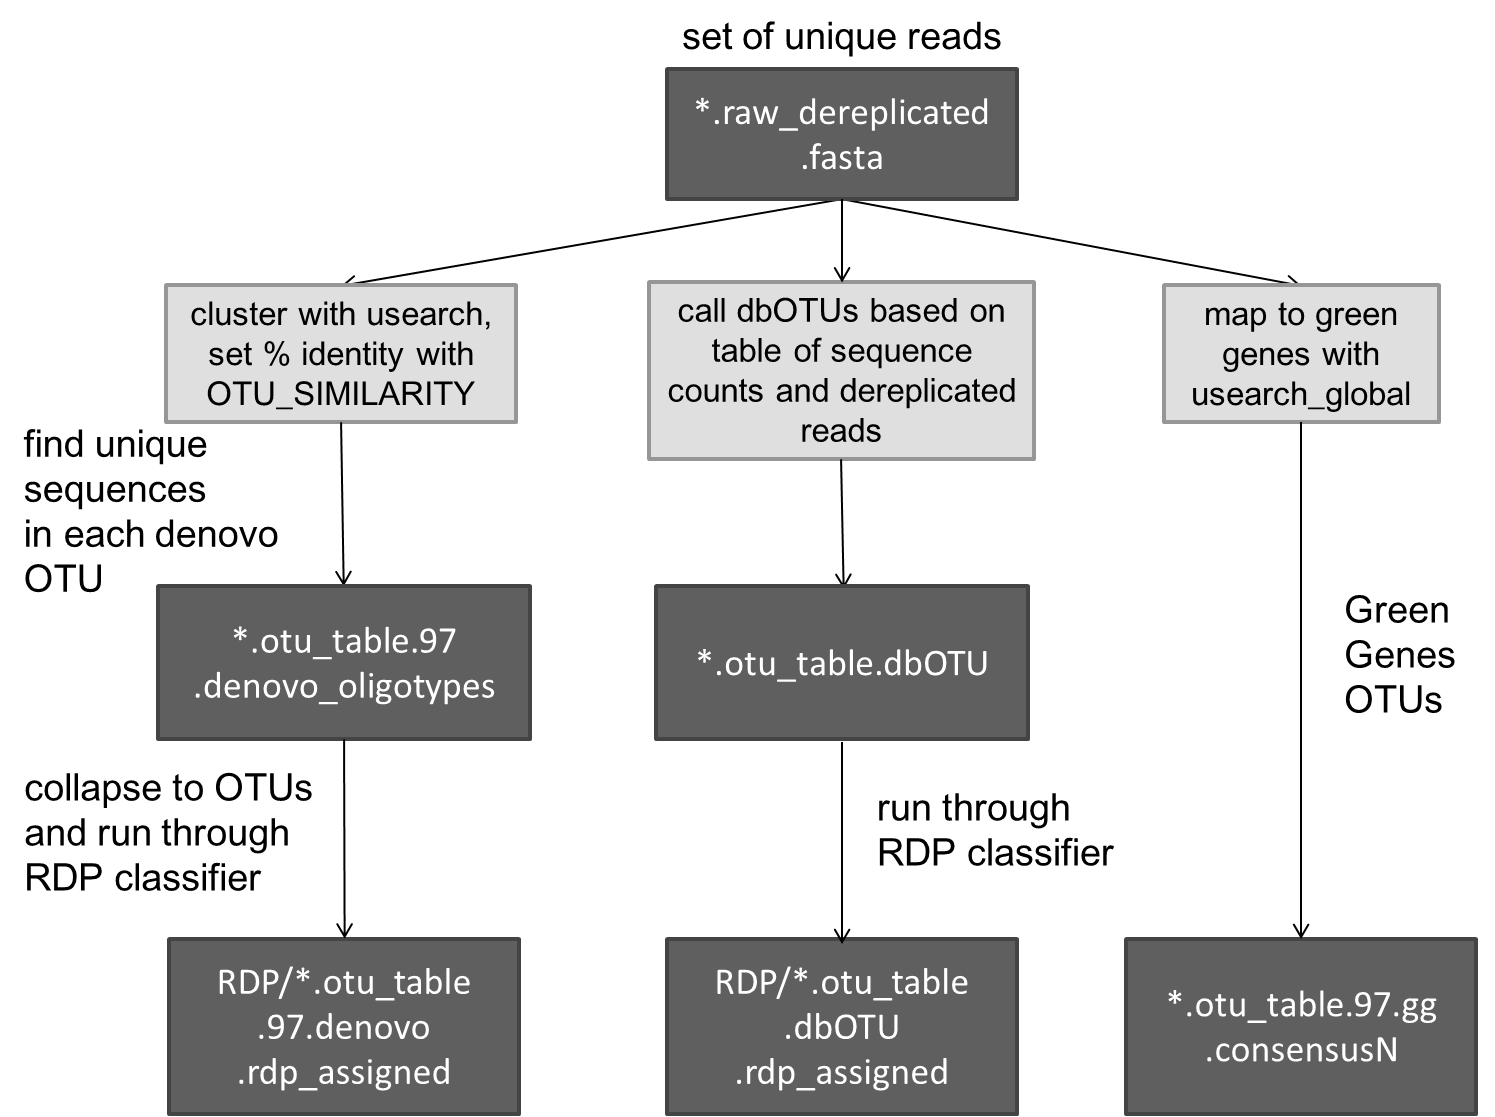
\includegraphics[width=0.8\textwidth]{figs/OTU_calling.png}
\caption{Schematic of OTU calling pipeline.}
\end{figure}


\subsubsection{\textit{de novo} OTU tables}
The dereplicated reads are clustered to within the specified sequence similarity percentage cut-off ({\tt OTU\_SIMILARITY}, default: 97) using {\tt usearch}.  Individual reads are assigned either as the OTU centroid or as a match. Centroids are labeled as 'OTU\_ID.0' and matches count from 'OTU\_ID.1' onwards.  These are separate oligotypes within the OTU 'OTU\_ID'. All oligotype counts are then collapsed to their respective OTU, resulting in a fully \textit{de novo} OTU table which can be found in the filename {\tt datasetID.otu\_table.*.denovo} where '{\tt *}' gets replaced by the OTU similarity cut-off.

\subsubsection{Closed-reference OTU table}
There are two types of database-referencing that are outputed from the pipeline by default.  The first is assignments from the Ribosomal Database Project (RDP), which returns probabilistic assignments.  The default probability cut-off below which an assignment is labeled as unidentified at a given taxonomic level is 0.5, but this can be set using a summary file parameter {\tt RDP\_CUTOFF}.  This OTU table can be found in the results sub-folder called 'RDP'.

The dereplicated reads are also aligned to a standard database (GreenGenes in the case of 16S sequences and UNITE in the case of ITS sequences).  In the case of GreenGenes, the database is determined based on the specified OTU similarity cut-off: e.g. {\tt 97\_otus.fasta} for {\tt OTU\_SIMILARITY} set to 97).  The alignment is performed using {\tt usearch}, and considers the top 10 hits.  Consensus assignments are then produced for the top 1, top 3, top 5 and top 10 hits (where a taxonomic level is only assigned a latin name if the top N hits from GreenGenes agree), and the corresponding OTU tables are output.  Thus, the OTU table called {\tt datasetID.otu\_table.*.gg.consensus10} contains latin names which are formed from a minimum consensus of the top 10 hits for each taxonomic level, where '{\tt *}' gets replaced by the OTU similarity cut-off.  Levels are left unidentified (e.g. '{\tt s\_\_}') if the consensus requirement is not met.  

Note that the database referencing process is one of the slower steps in the pipeline, so if you only care about RDP, you can skip the GreenGenes assignments steps by setting the parameter {\tt GG\_ALIGN} to {\tt False} in the summary file.  Similarly, for ITS sequences, you can skip the UNITE assignments steps by setting the parameter {\tt UNITE\_ALIGN} to {\tt False}.

\subsubsection{Open-reference OTU table}
{\tt DEPRECATED:} The pipeline no longer produces open-reference OTUs. 

If any reads in the dereplicated sequences do not align to GreenGenes/UNITE to within the specified similarity cut-off, they are clustered with the desired similarity cut-off using {\tt usearch}, and appended to the GreenGenes/UNITE closed-reference table to produce a full, open-reference OTU table (which combines GreenGenes-referenced and \textit{de novo} OTUs) at the desired similarity cut-off, with filename {\tt datasetID.otu\_table.gg.*.open\_ref}.

\subsubsection{Oligotypes}
The OTU calling process automatically assigns separate IDs to unique sequences within OTUs (termed 'oligotypes' by some).  These offer a greater level of granularity.  For example, if sequences A, B and C are all the same OTU, called OTU1 (and the centroid is sequence A), these would be relabeled 'OTU1.0', 'OTU1.1' and 'OTU1.2'.

There is currently one such table output: the full \textit{de novo} oligotype table (where sequences are labeled according to a fully \textit{de novo} OTU clustering process) - \\{\tt myDataset.otu\_table.N.denovo\_oligotypes}

\subsection{Taxon abundances and diversities}
...

\subsection{PiCRUST}
OTU tables are sent off to a second node for metagenome prediction using PiCRUST.  It will return predicted abundances of the different KEGG modules, including abundances of pathways collapsed at each different level of abstraction in the KEGG hierarchy.  These abundances are encoded in BIOM format tables and can be found in the results directory.  Stacked bar plots of the different KEGG module abundances on a per sample basis, as produced by QIIME, are also added to the results directory. 

\subsection{Downstream analysis}
...

\section{Resulting 16S features}
The resulting 16S features are returned in a features object, computed using the {\tt Features.py} module.  This object can be found in pickled form in the results directory, under the filename {\tt pickled\_features.pkl}.  The pickled object can be loaded in Python as follows:
\begin{verbatim}
import pickle

with open('pickled_features.pkl', 'r') as fid:
    features = pickle.load(fid)
\end{verbatim}
The resulting {\tt features} object has the full feature vectors for each sample stored in {\tt features.feature\_vectors}, which is a {\tt dict} whose keys are the sample IDs (the same as those specified in the provided metadata file, and in the resulting OTU table).  Thus, the feature vector for sample 'A' can be found in {\tt features.feature\_vectors['A']}.  The name of the feature at index $i$ of the feature vectors can be accessed from {\tt features.feature\_descriptions[i]}.  The full list of features includes:

\begin{itemize}
	\item OTU abundances.
	\item Oligotype abundances (in the form OTU1.1, OTU 1.2, OTU 1.3, ..., where OTU1.1 represents oligotype 1 of OTU 1).
	\item KEGG module abundances, at levels 1, 2, 3 and 4.
	\item L/R phylogenetic features.
\end{itemize}

\section{Source code - Python modules}
\subsection{Modules}
\begin{itemize}
  \item {\tt Formatting.py} - Module to house miscellaneous formatting methods, e.g. conversion from classic dense format to BIOM format, OTU table transposition, etc.
	\item {\tt QualityControl.py} - Methods for quality control diagnostics on a dataset.
	\item {\tt preprocessing\_16S.py} - Methods and wrappers for raw 16S sequence data processing.
	\item {\tt CommLink.py} - Communications module between the various processing nodes.  Links processing node, PiCRUST server and QIIME/plotting server.  Manages inbox listeners for each type.
	\item {\tt Taxonomy.py} - Methods for taxonomy-related feature extraction and analytics.  Includes functions for things like:
		-adding latin names to a GreenGenes-referenced OTU table
		-collapsing abundances at different taxonomic levels
	\item {\tt Phylogeny.py} - Methods for phylogenetic feature extraction, e.g. left/right (LR) abundance ratios at each node of a phylogenetic tree.
	\item {\tt Analytics.py} - Generic statistical analysis tools, e.g. Wilcoxon tests across all available taxa.
	\item {\tt Regressions.py} - Performs different types of regressions \textit{en masse}.
	\item {\tt UserInterface.py} - Routines for preparing JSON files and other required files for use on the UI/dashboard.
	\item {\tt DepositDB.py} - Methods for depositing data into the database.
\end{itemize}

\begin{figure}
\centering
	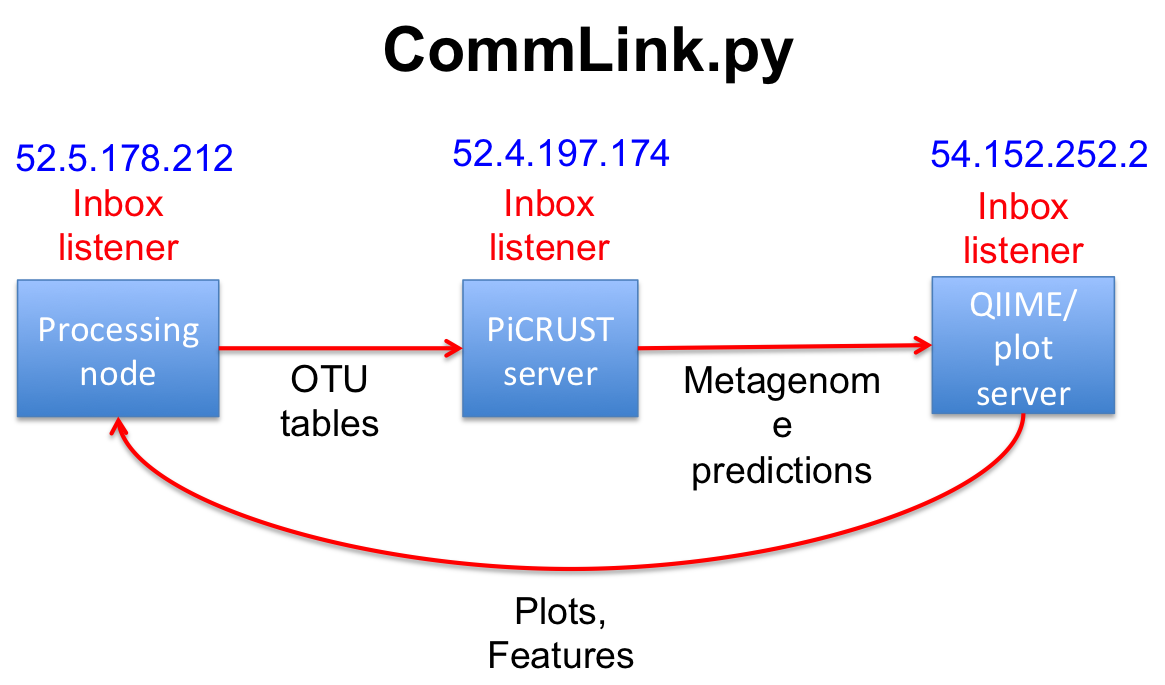
\includegraphics[width=0.8\textwidth]{figs/CommLink.png}
\caption{Work flow managed by CommLink.py.}
\end{figure}

\subsection{Scripts and routines}
\begin{itemize}
	\item {\tt Master.py} - Master script that calls relevant processing pipelines, e.g. {\tt raw2otu.py}.
	\item {\tt raw2otu.py} - Pipeline for converting raw 16S FASTQ sequence files to OTU tables.  Handles parallelization requirements in these processing steps automatically.  Takes as input a directory that contains a summary file and the raw data.
\end{itemize}

\section{Troubleshooting}
Standard error ({\tt stderr}) and standard out ({\tt stdout}) are directed to the directory {\tt /home/ubuntu/logs}.  Errors will appear in the {\tt stderr} file for the corresponding datasets.  In addition, file outputs from each step of the pipeline can be found in {\tt /home/ubuntu/proc/datasetID\_proc\_16S}, which can help to diagnose errors.  Common sources of errors or difficulties include:

\begin{itemize}
\item Bad formatting of the summary, barcodes, or primers file.  There should be no white spaces, and columns should be tab-delimited.  If you created the file in Excel, it may have carriage return or other non-linux formatting characters that introduce difficulties.  Safest is to go from a previous summary file template, or to create it manually.
\item Typos in a 16S attribute key-value pair in the summary file.
\item Incorrect ASCII encoding specified.  Check whether 33 or 64 using {\tt usearch8 -fastq\_chars yourFASTQfile.fastq}.  Default is 33, so if left unspecified and the file is ASCII base 64, quality trimming will fail.
\item For ITS sequences, the RDP classifier often runs out of RAM when loading the UNITE database.  This is usually what happened if you find {\tt RDP\_classification.txt} to be empty in the relevant folder in {\tt /home/ubuntu/proc}.  If you rerun the pipeline several times, have checked everything else and keep encountering this problem, you may need a node with more RAM to do your processing.
\item If you specify a file containing a list of FASTQ/FASTA files for the raw reads, make sure the file paths are relative to the directory hosting the summary file.
\end{itemize}
\end{document}  